% Standalone build of the block diagram that appears as a figure in the paper.
% The body is the same tikzpicture, so the two cannot drift apart by accident.
%   tectonic -X compile fig_architecture.tex
\documentclass[border=4pt]{standalone}
\usepackage{tikz}
\usepackage{xcolor}
\usetikzlibrary{arrows.meta,positioning,fit,backgrounds,calc}

\definecolor{segfill}{HTML}{DCE9F7}
\definecolor{segline}{HTML}{2A78D6}
\definecolor{labfill}{HTML}{E6E0F5}
\definecolor{labline}{HTML}{6B4FBB}
\definecolor{iofill}{HTML}{ECECE8}
\tikzset{
  blk/.style={draw, rounded corners=2pt, align=center, inner sep=3.2pt,
              font=\scriptsize, minimum height=7.5mm, line width=0.5pt},
  seg/.style={blk, fill=segfill, draw=segline},
  lab/.style={blk, fill=labfill, draw=labline},
  io/.style={blk, fill=iofill, draw=black!55},
  op/.style={draw, circle, inner sep=0.8pt, font=\scriptsize, line width=0.5pt,
             fill=segfill, draw=segline},
  fl/.style={-{Latex[length=1.6mm,width=1.4mm]}, line width=0.5pt, draw=black!70},
  note/.style={font=\tiny, text=black!60, align=center},
}

\begin{document}
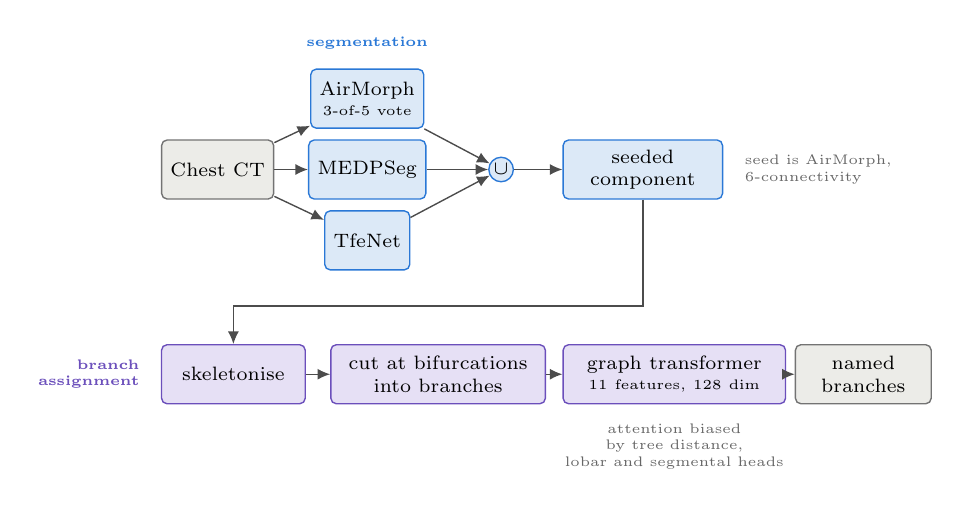
\begin{tikzpicture}

% ---- row 1, the segmentation front end
\node[io] (ct) {Chest CT};
\node[seg] (mp) at ($(ct)+(19mm,0)$) {MEDPSeg};
\node[seg] (am) at ($(mp)+(0,9mm)$) {AirMorph\\[-1pt]\tiny 3-of-5 vote};
\node[seg] (tf) at ($(mp)+(0,-9mm)$) {TfeNet};
\node[op]  (or) at ($(mp)+(17mm,0)$) {$\cup$};
\node[seg, text width=18mm] (lcc) at ($(or)+(18mm,0)$) {seeded\\component};
\node[note, right=1.5mm of lcc, text width=21mm, align=left]
  {seed is AirMorph,\\6-connectivity};
\draw[fl] (ct) -- (am); \draw[fl] (ct) -- (mp); \draw[fl] (ct) -- (tf);
\draw[fl] (am) -- (or); \draw[fl] (mp) -- (or); \draw[fl] (tf) -- (or);
\draw[fl] (or) -- (lcc);

% ---- row 2, branch assignment. The connector runs in a clear channel between
% the rows, so it crosses no block.
\node[lab, text width=16mm] (sk) at ($(ct)+(2mm,-26mm)$) {skeletonise};
\node[lab, text width=25mm] (pc) at ($(sk)+(26mm,0)$) {cut at bifurcations\\into branches};
\node[lab, text width=26mm] (gt) at ($(pc)+(30mm,0)$)
  {graph transformer\\[-1pt]\tiny 11 features, 128 dim};
\node[io, text width=15mm] (out) at ($(gt)+(24mm,0)$) {named\\branches};
\draw[fl] (sk) -- (pc); \draw[fl] (pc) -- (gt); \draw[fl] (gt) -- (out);
\node[note, below=1.2mm of gt, text width=32mm]
  {attention biased by tree distance,\\lobar and segmental heads};

\coordinate (ch) at ($(lcc.south)+(0,-13.5mm)$);
\draw[fl] (lcc.south) -- (ch) -| (sk.north);

% ---- which stage is which
\node[note, above=1.2mm of am, text width=30mm, text=segline]
  {\textbf{segmentation}};
\node[note, left=1.5mm of sk, text width=13mm, align=right, text=labline]
  {\textbf{branch\\assignment}};
\end{tikzpicture}
\end{document}
